\section{Übersicht Gesamtsystem}\label{kap:ausw}
 \subsection{Inbetriebnahme}
 \subsubsection{Hardware Voraussetzungen}
 Voraussetzung für den Betrieb ist ein Raspberry Pi 2 oder 3. Außerdem ist eine Erweiterungsplatine \chphl{PiFace Digital2 \cite{URL:PiFaceDigital2}} erforderlich. Diese muss vor dem ersten Start auf die GPIO-Kontakte des Raspberry Pi aufgesteckt werden. Eine Funktion ohne das Hardwaremodul ist Grundsätzlich möglich, jedoch scheint ein Betrieb ohne Hardwareschnittstelle ohne Sinn. Die Software ist so konzipiert, dass auch andere Hardware-Module denkbar sind, eine Implementierung hierfür fehlt jedoch bislang.     
 \subsubsection{Software Voraussetzungen}
 Für den Betrieb wird ein Linux Betriebssystem vorausgesetzt. Hierfür kann das angepasstes Raspbian \cite{URL:Raspian} Image genutzt werden, welches auf der beigelegten DVD zu finden. Falls auf der SD Karte bereits ein Linux Betriebssystem installiert ist, kann das Arbeitsverzeichnis des Projekts auch einfach auf den Raspberry Pi übertragen werden. Ein Git Auszug hiervon ist ebenfalls auf der beigelegten DVD. Sollte die Wahl der Distribution auf eine andere als Raspbian Strech \cite{URL:Raspian} fallen, so muss das Projekt aus den Quellen übersetzt werden. In jedem Fall ist es nötig dass SPI aktiviert wird. Dies geschieht am einfachsten über das Raspberry Pi Konfigurationsprogramm. \texttt{sudo raspi-config} 
 \subsubsection{Kompilieren des Projekts}
 Ein kompilieren des Projekts ist nur erforderlich, wenn das Projekt auf einem anderen Betriebssystem als Raspian Strech \cite{URL:Raspian} verwendet werden soll, oder wenn Änderungen am Quellcode vorgenommen werden sollen.  
 Dafür muß zunächst eine SSH Verbindung zum System herstellt werden. Das Projekt sollte daraufhin auf das System übertragen werden. Die Empfohlene Vorgehensweise hierfür ist, das GIT Repository über eine aktive Internetverbindung auf den Rasperry Pi zu klonen. \texttt{git clone https://github.com/dajuly20/ControlPi}. Um alle Abhängigkeiten dann automatisch zu installieren, kann nachfolgend genannte Installationsscript verwendet werden: \texttt{./start\_pull\_and\_build.sh}. Sollte keine Internetverbindung bestehen, können die auf der DVD mitgelieferten Bibliotheken auch manuell installiert werden. 
 Eine Liste der benötigen Abhängigkeiten findet sich im \nameref{chp:anhang}.  
 \subsubsection{Inbetriebnahme unter Raspbian Strech}
 Sollte auf dem Raspberry Pi bereits ein Version von Raspbian in der Version Strech installiert sein, so genügt es den Projektordner auf den Raspberry Pi zu übertragen. Hierfür dient entweder der Ordner \texttt{ControlPi} auf der beigelegten DVD, oder das GIT Repository des Projekts, welches mittels  \texttt{git clone https://github.com/dajuly20/ControlPi} auf den Raspberry Pi übertragen werden kann. Um sicherzustellen dass es sich um die aktuellste Version handelt, sollte das Projekt mit \texttt{git pull} auf den neusten Stand gebracht werden. Daraufhin kann mit \texttt{./start\_manual.sh} die Funktion überprüft werden. Dabei sollte der Benutzer in den Gruppen \texttt{spi} sowie \texttt{gpio} sein. Letztlich sollte das Projekt als Systemservice eingerichtet werden. Hierfür ist das Script \texttt{./start\_as\_service.sh} dienlich. Es wird hier neben dem eigenen Systemservice auch ein Apache2 Webserver mit in Betrieb genommen.
 \subsubsection{Ermittlung der IP - Adresse}\label{chp:ausw:ip}
 Nachdem der Systemservice läuft, muss nun ermittelt werden wie ein Zugriff auf die Weboberfläche erfolgen kann. Wenn der Raspberry Pi in ein bestehendes Netzwerk integriert wird, kann dies in der Oberfläche des verwendeten Internetrouters nachgesehen werden. Sofern dieser dies unterstützt, kann auch der Hostname des Raspberry Pi für den Zugriff verwendet werden. Der Hostname im mitgelieferten Raspian-Image lautet \texttt{ControlPi3}. Der Standard bei einem offiziellen Raspbian Image ist \texttt{raspberrypi}. 
 \subsection{Funktionstest}
 \subsubsection{Testen der Betriebsbereitschaft}
 Im Auslieferungszustand ist ein zu Testzwecken bereits ein Steuerungsprogramm enthalten. Dieses lässt die LED an Ausgang 6 durch einen sich selbst aufrufenden Timer blinken. Zudem ist in diesem Testprogramm den Ausgängen \texttt{0} sowie \texttt{1} der Wert der Eingänge \texttt{0} beziehungsweise \texttt{1} zugewiesen. Ein Drücken der in \autoref{img:PiFaceDigital2} gezeigten Taster S0 oder S1 sollte also ein Leuten der entsprechenden LED zur Folge haben. Wie auch bei den Tastern, werden auch die LEDs von rechts nach links durchnummeriert und sind den jeweiligen Ausgängen örtlich zugeordnet. Da an den Ausgängen \texttt{0} und \texttt{1} zudem Relais angeschaltet sind, sollte ein Zustandswechsel auf diesen Ausgängen außerdem in Form eines Klickgeräusches hörbar sein. 

 
 \begin{figure}[H]
 	\begin{center}
 		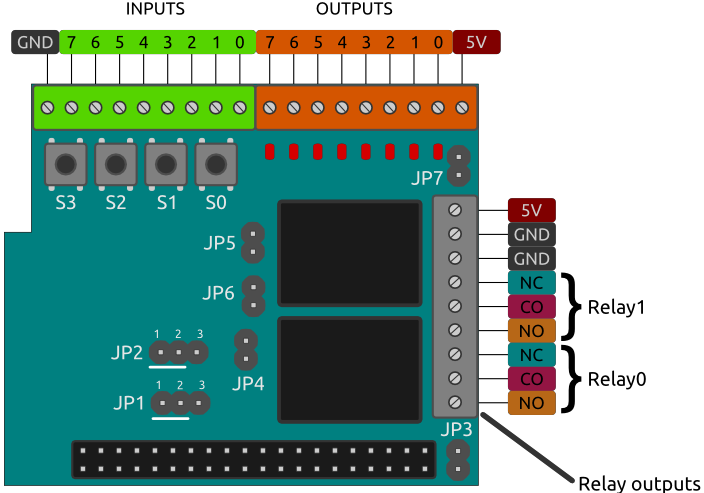
\includegraphics[width=0.95\textwidth]{./images/pifacedigital2_diagram.png}
 		\caption[Darstellung eines PiFace Digital 2]{Darstellung eines PiFace Digital 2 \cite{URL:Pfd}}
 		\label{img:PiFaceDigital2}
 	\end{center} 
 \end{figure}	

 \subsubsection{Aufruf der Weboberfläche}\label{chp:FrontendUebersicht}
Ist der Hostname oder die IP Adresse des Raspberry Pi ermittelt (siehe Abschnitt \ref{chp:ausw:ip} \nameref{chp:ausw:ip}), kann dieser im Internetbrowser aufgerufen werden. Bei Verwendung des beigelegten Raspbian Images wäre der Aufruf \texttt{http://ControlPi3}. \autoref{img:FrontendUebersicht} zeigt die Übersichtsseite der Steuerung. In der Mitte befindet sich eine Abbildung vom aktuell verwendeten Steuerungsprogramm, während an den Seiten die Zustände ein und Ausgänge angezeigt werden. Die Drop-Down Menüs oberhalb, ermöglichen es die gewünschte Ein- bzw. Ausgangsentität auszuwählen. Handelt es sich bei der ausgewählten Entität um einen Eingang, so wird anstelle einer LED ein Taste eingeblendet. Der Zustand kann dann, bei entsprechender Berechtigung (siehe \chpref{chp:ums:websock:auth} ), durch anklicken verändert werden.  

 \begin{figure}[H]
	\begin{center}
		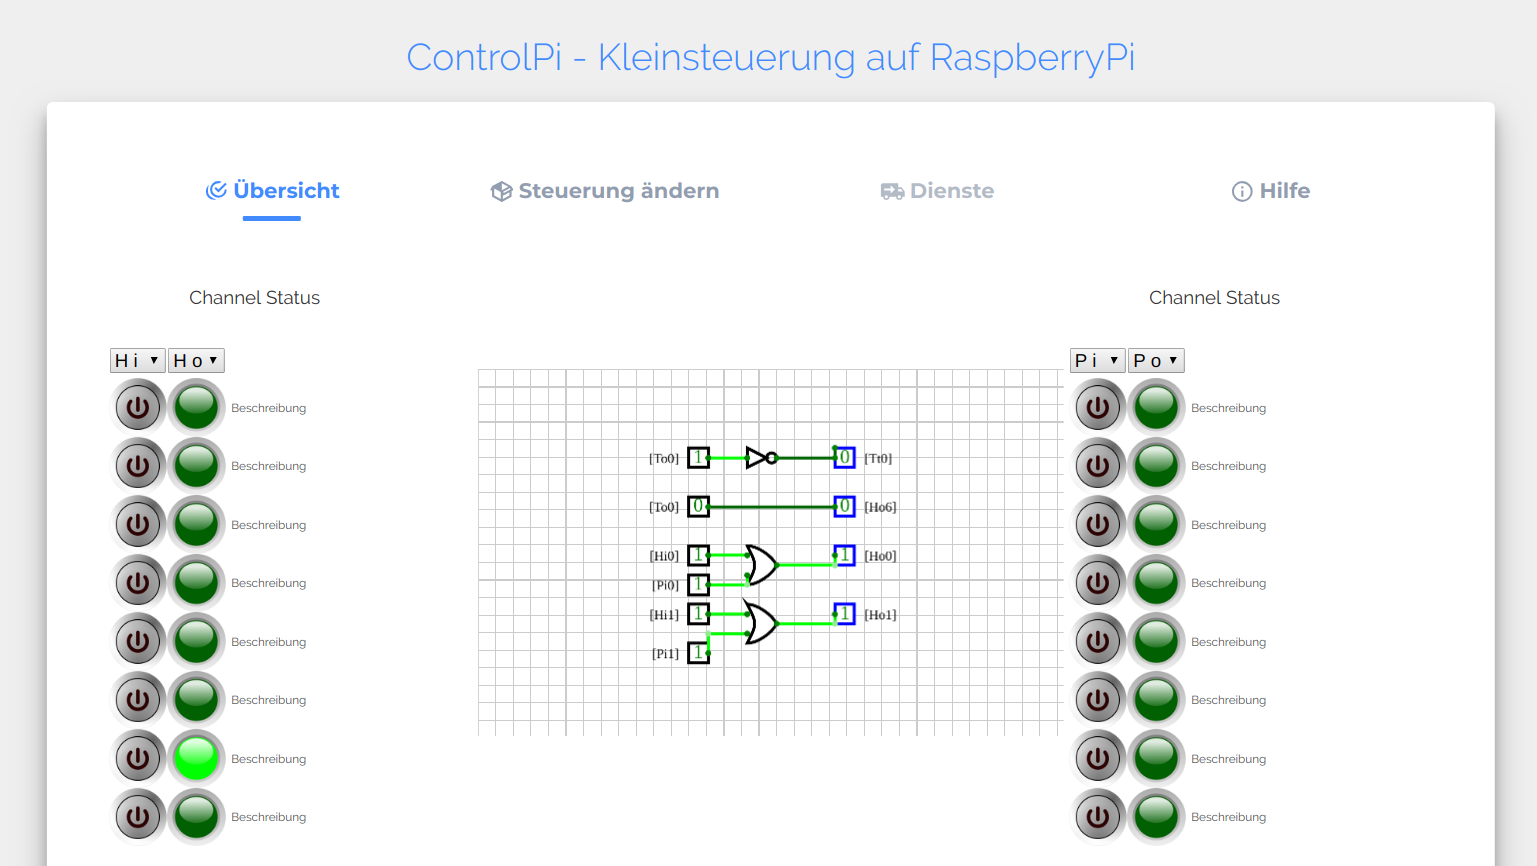
\includegraphics[width=0.95\textwidth]{./images/FrontendUebersicht.png}
		\caption{Darstellung Frontend Übersicht}
		\label{img:FrontendUebersicht}
	\end{center} 
\end{figure}

\subsubsection{Erstellen eines Steuerungsprogramms}

Um ein Steuerungsprogramm zu erstellen, muß zunächst der Tab \texttt{Steuerung ändern} angewählt werden. Nun erscheint der in \autoref{img:FrontendAenderung} abgebildete Logik-Editor CicuitVerse \cite{URL:CircuitVerse}. Sollte die vorhandene Logikschaltung nicht sofort sichtbar sein, muss die Zeichenfläche zuerst durch klicken auf das Fadenkreuz-Symbol in den Mittelpunkt gerückt werden. Soll nun eine komplett neue Schaltung gezeichnet werden, kann die Zeichenfläche durch den Unterpunkt \texttt{Clear Project} im Drop-Down Menü \texttt{Project} bereinigt werden. Alle verfügbaren Bauteile befinden sich im Bauteil-Menü auf der linken Seite. Dieses ist in die Kategorien \texttt{Input} \texttt{Output} und \texttt{Gates} unterteilt, welche sich durch anklicken aufklappen lassen. Möchte man ein Bauteil auf die Zeichenfläche schieben, so muss dieses angeklickt und der Cursor auf die  Zeichenfläche bewegt werden. Ein erneutes Klicken lässt das Bauteil  an der gewählten Position fallen. Die Bauteile werden schließlich mittels Drag and Drop mit einander Verbunden. Werden Timerbausteine angeklickt, so  lassen  sich die Einschalt und Ausschalt- Verzögerungszeiten im Menü \texttt{Properties} einstellen. Es gilt zu beachten, dass Ausgänge jeweils nur einmal vorkommen dürfen. Gibt es mehrere Möglichkeiten in denen ein Ausgang aktiv werden soll, empfiehlt sich die Verwendung eines Und- bzw. Oder- Gates.  Nach Vollendung des Steuerungsprogramms, kann die Steuerung mit dem Menüpunkt \texttt{Save \& Export}, welcher sich im Menü \texttt{Project} befindet, übernommen und getestet werden. Eine Überprüfung auf Richtigkeit des Steuerungsprogrammes erfolgt nicht. Deshalb sollte der Info-Kasten \texttt{Backend Status} im Auge behalten werden. Falls ein Fehler mit dem Steuerungsprogramm auftritt, wird dieser dort angezeigt. 
	

 \begin{figure}[H]
	\begin{center}
		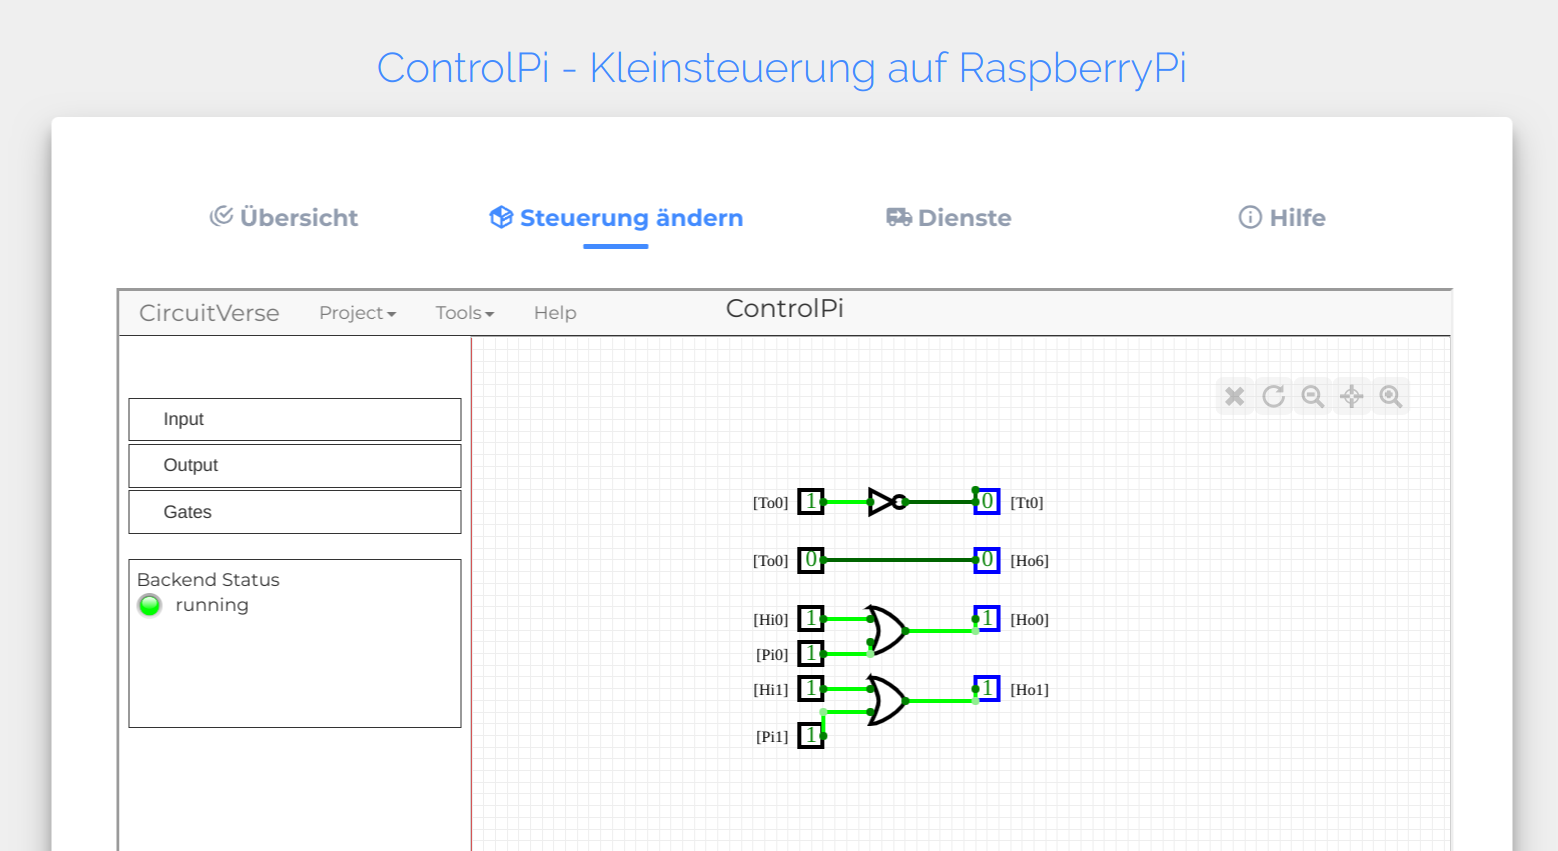
\includegraphics[width=0.95\textwidth]{./images/FrontendAendern.png}
		\caption{Darstellung Logik Editor}
		\label{img:FrontendAenderung}
	\end{center} 
\end{figure}	


 \subsection{Bugs}
 Zum derzeitigen Stand sind noch einige Probleme enthalten auf die nachfolgend eingegangen wird. Als  erstes sei hier zu nennen, dass die Reihenfolge in welcher das Backend über die Zeilen des erzeugten Steuerungsprogramms Iteriert unter bestimmten Voraussetzung Probleme bereitet. So wird der Wert eines Ausgangs unter noch nicht näher bekannten Umständen erst mit der nächsten Iteration des Logikprogramms übernommen. Dies könnte durch generelles doppeltes iterieren behoben werden, was allerdings die Performance vermindert.
 
 \subsection{Fazit}
 \subsection{Ausblick}
 Die Steuerung Funktioniert in den meisten Fällen ohne Probleme, ist jedoch noch nicht über ein frühes Betastadium hinaus. Es bedarf nun Feldtests um weitere Bugs in der Software aufzuspühren. Außerdem sind noch einige Funktionserweiterungen Denkbar. Zuerst anzuführen wäre hier die Kopplung zweier Geräte. Die Grundvoraussetzungen hierfür sind durch die Implementierung  von WebSockets bereits geschaffen. Entweder müsste hier eine Mittelschicht geschrieben werden, welche die zwei WebSocket Server auf den beiden Geräten miteinander kommunizieren lässt. Etwas eleganter jedoch wäre die Implementierung eines WebSocket Clients in das Backend. Mit einer angepassten Konfigurationsdatei könnte das Backend sich so zu einem anderen Gerät verbinden um dessen Virtuelle Ein und Ausgänge auch am lokalen Gerät nutzbar zu machen. WebSockets haben durch die persistente Verbindung sehr gutes Verhältnis zwischen Overhead und Payload und sollten somit eine recht geringe zeitliche Verzögerung ermöglichen. Die Erfahrung von der Verbindung zwischen Web-Frontend und Backend zeigen kaum merkliche Verzögerungszeiten. Eine Weitere Funktion über welche nachgedacht wurde, ist ein anlegen von Unterstromkreisen. Somit könnten zum Beispiel Blinkerbausteine oder \texttt{Stromstoßschalter}, das sind Bauteile die ihren Logikzustand durch einen Eingangsimpuls wechseln, realisiert werden. Dabei würde die Implementierung abstrahiert und die Übersichtlichkeit erhöht. Ebenfalls denkbar wäre die Zusammenfassung der Timer Ein- und Ausgänge in ein einziges Bauteil. Die Umsetzung beim Export könnte hierbei beibehalten werden. 
  
 Kopplung mehrerer Geräte;
 Beschriftung der Ein Ausgänge in der Web Oberfläche. 
 Shortcuts z.B. für Blinker
 Set und Reset für Timer,
 Set und Reset für Relays.
 Änderung des Passworts für die Weboberfläche.
 
 
 
\clearpage